\section{Proposed Method}
\label{sec:method}

A complete pipeline of Shape-Constrained Neural Network (SCNN) is illustrated in Figure~\ref{FigSCNN}.
The framework is trained end-to-end and consists of three key components:
1) a multi-task neural network based on FCN,
2) proposed joint max pooling and
3) local optimizing strategy to fuse the multi-outputs into final segmentation mask.
%

Given an input image, the first part is a multi-task FCN which separately predicts objectness scores and shape parameters maps (Sec.~\ref{sec:multi-task-fcn}).
Then two branches integrate with each other by a joint max pooling layer (Sec.~\ref{sec:joint-max-pooling}) and a local fusion step to finally predict the shape-constrained segmentation (Sec.~\ref{sec:fusion}).

\subsection{Multi-task FCN}
\label{sec:multi-task-fcn}

The architecture of our multi-task learning network is shown in Figure~\ref{FigMTN}.
It simultaneously predicts an objectness map $P$ and several auxiliary maps $\{T_k\}_{k=1,\ldots,K}$ as complementary information.
The feature extracting part is shared and based on the publicly available DeepLab model~\cite{Chen2014a}, which introduces zeros into the filters to enlarge its Field-of-View.
Subsequently, the feature maps extracted by last shared convolution layer are fed into two individual branches.
In each branch, successive two convolution layers, respectively with kernel size of $3\times3$ and $1\times1$, are applied to the input feature maps, then an upsampling layer restores the resolution of predictions to the input image size.
During training, the parameters of shared layers are jointly optimized, while the parameters of two branches are updated independently.

\begin{figure}
    \begin{center}
        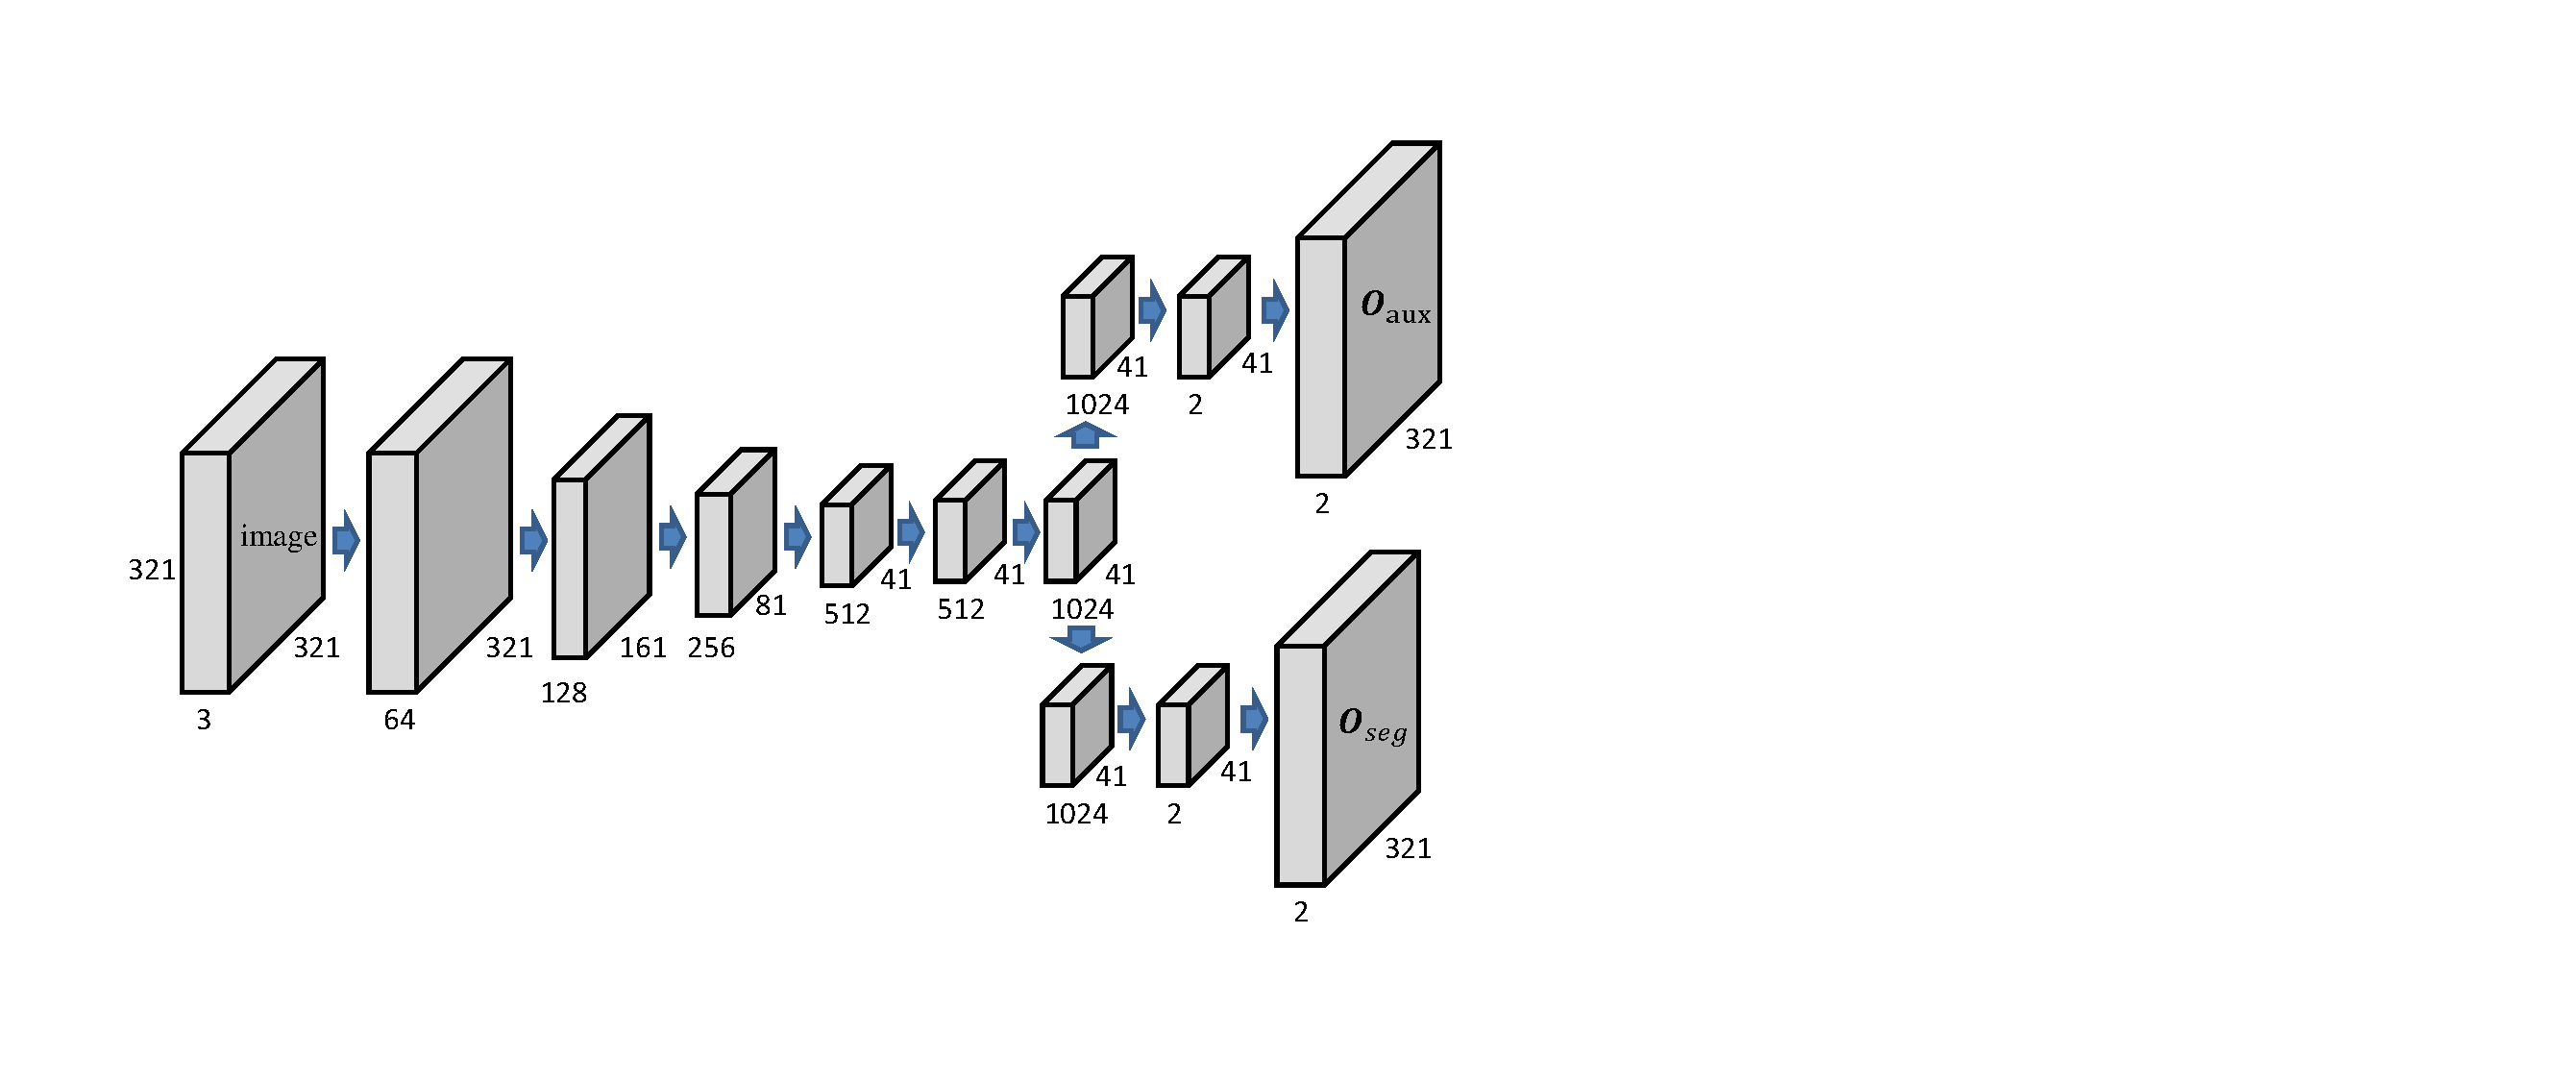
\includegraphics[width=3.3in]{figures/FigMTN.pdf}
    \end{center}
    \caption{Architecture of multi-task neural network based on FCN. \cxj{I would sugest using real images as input and output.}}
    \label{FigMTN}
\end{figure}
Instead of directly predicting contour probabilities in \cite{Chen2016a,Xu2016}, we choose the parameterized expression of objects shape as complementary information, which emphasizes more on the overall shape of objects to be segmented.
For example in our task for vesicle segmentation, the ellipse shape is selected as our prior shape knowledge and formulated by $5$ parameters: $\{\theta, \mu_c, \nu_c, a, b\}$.
$\theta$ is the rotated angle of the major axis from $x-$axis.
$(\mu_c, \nu_c)$ are the coordinates of the center.
And $a$, $b$ are respectively the lengths of the major and minor axis.
With these definitions, $K$ is set to be $5$ and each $T_k$ corresponds to one parameter.
At each pixel $i$, the predicted vector $\{T_{1,i},\ldots,T_{5,i}\}$ describe the shape of a nearest object.
For better regression, the predicted parameters are further normalized by image width $W$ and height $H$ so that they fall in $[0,1]$:
\begin{eqnarray}\label{EqMax}
\begin{aligned}
\{T_{1,i},\ldots,T_{5,i}\} = \{\theta,\frac{\mu-\mu_c}{W},\frac{\nu-\nu_c}{H},\frac{a}{H},\frac{b}{H}\}
\end{aligned}
\end{eqnarray}
where $(\mu, \nu)$ are spatial coordinates of pixel $i$.

For an input image, The objective function of our multi-task FCN is defined by:
\begin{eqnarray}\label{EqLoss}
\begin{aligned}
L(P,\{T_k\}) =& \frac{1}{N}(\sum_{i}L_{cls}(P_i,P^*_{i})+\\
&\lambda\sum_{i}\sum_{k}p^*_{i}L_{reg}(T_{k,i},T^*_{k,i}))\\
\end{aligned}
\end{eqnarray}
where $N$ is the total number of pixels.
$P^*_i$ and $T^*_{k,i}$ are the ground truth of objectness score and shape parameters at pixel i.
The classification loss $L_{cls}$ is the soft-max loss and regression loss $L_{reg}$ is defined by
\begin{eqnarray}
\label{EqSmoothL1}
\begin{aligned}
L_{reg}(x) =\left\{\begin{array}{cc}
0.5x^2&if~|x|<1\\
|x|-0.5&else\\
\end{array}\right.
\end{aligned}
\end{eqnarray}
which is the smoothed $L_1$ loss for robust regression in \cite{Ren2015}.

Especially in Eq.~\ref{EqLoss}, we only consider the regression loss with positive $P^*_i$, because most $T_{k,i}$ along with negative $P^*_i$ will be abandoned in next section by proposed joint max pooling.
And $\lambda$ is a balancing weight between $L_{cls}$ and $L_{reg}$.

\subsection{Joint Max Pooling}
\label{sec:joint-max-pooling}

Obtained from two individual branches of multi-task FCN, objectness and auxiliary maps are raw and uncorrelated \bobo{Is it too strict by using 'uncorrelated' because of the shared feature in FCN}.
Usually in an auxiliary map, only predicted shape parameter in central area of an object satisfy the requirement of accuracy.
This is caused by intrinsic challenge of different perception field needed by different position to explore the complete shape of a nearest object.
To this end, we introduce a novel joint max pooling (JMP) to improve the accuracy of auxiliary predictions in border area of objects, which can effectively improve the performance of next optimizing step.
Different from conventional max pooling, our JMP simultaneously takes two maps as inputs and pools one with the other one.
Its back propagation can further benefit both inputs by exploring the inherent association between inputs.

A conventional pooling operation can expressed as
\begin{eqnarray}\label{pooling}
\begin{aligned}
y_{j} = \sum_{i\in \mathcal{N}_{j}} \omega_{i}x_{i}
\end{aligned}
\end{eqnarray}
where $\mathcal{N}_{j}$ is a neighbor region of pixel $j$ according to the sliding window, and $\omega_{i}$ is the weight of pixel $i$.
For traditional max pooling, $\omega_i \in \{0,1\}$ is a binary indicator for that if $x_i$ is the maximum in the local region.
There is only one pixel in the neighborhood has $\omega=1$ and all the others have $\omega=0$.
For an average pooling, all pixels in the local window take the identical weight $\omega=\frac{1}{N}$, where $N$ is the total number of pixels in the local region $\mathcal{N}$.
Intuitively, $\omega$ acts like an $``$indictor" determining which $x$ should be propagated to next layer.

\begin{figure}
    \begin{center}
        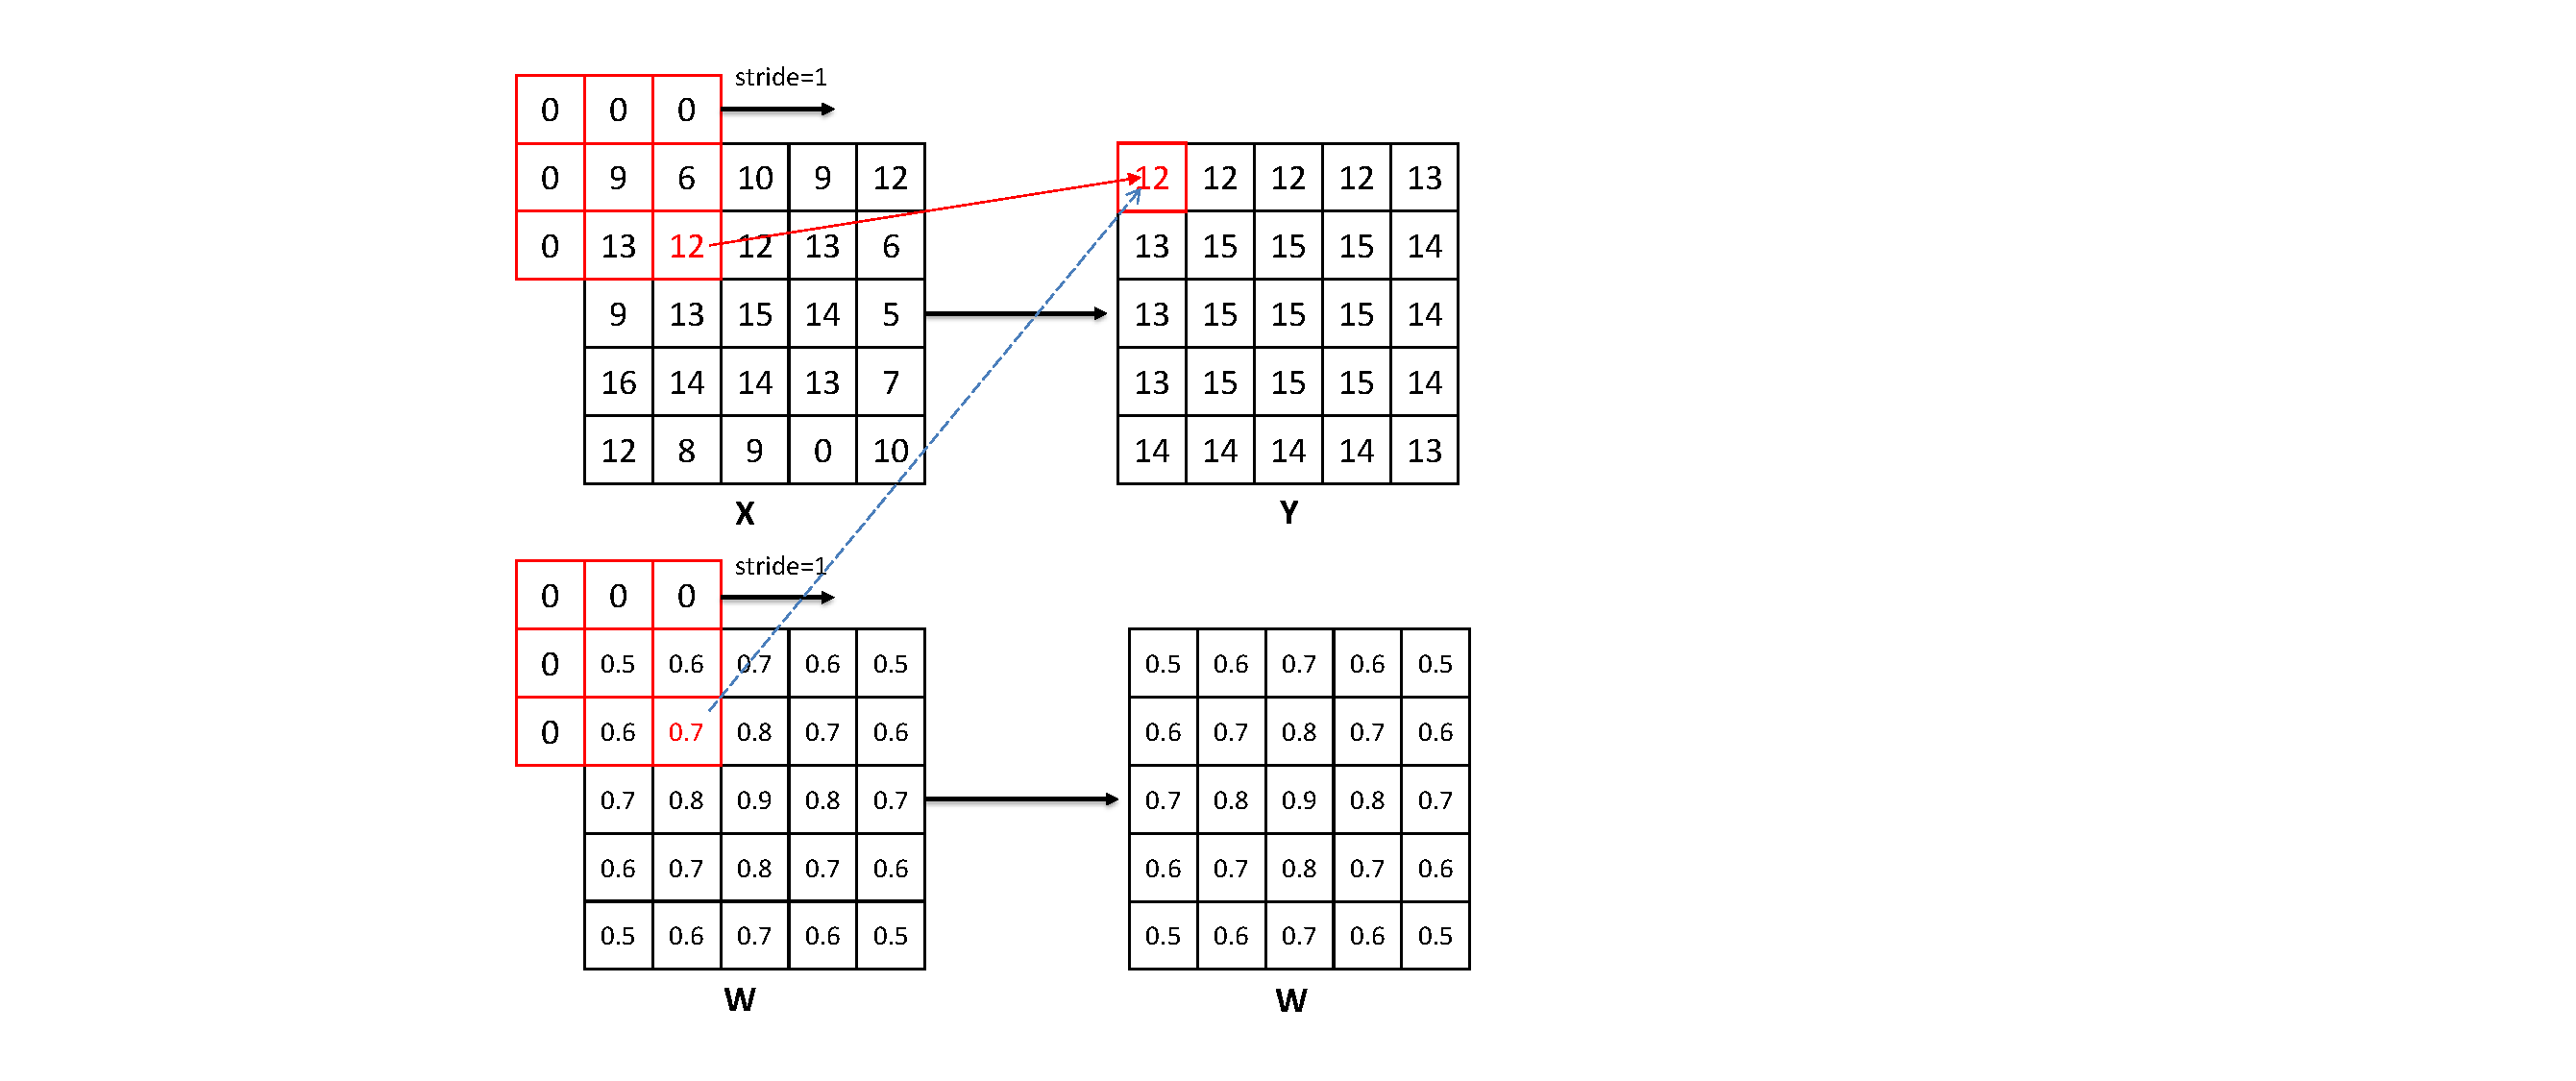
\includegraphics[width=3.4in]{figures/FigJMP.pdf}
   %\includegraphics[width=0.8\linewidth]{egfigure.eps}
    \end{center}
    \caption{An example of joint max pooling.
        Two windows of same size synchronously slide on $\mathbf{X}$ and $\mathbf{W}$.
       The elements in top window will be propagated the element under the indicator of bottom window.}
    \label{FigJMP}
\end{figure}

Based on this observation, we proposed a joint max pooling layer \bobo{change a name?} by learning $\omega$ independently, rather than from $x$.
Explicitly, our joint max pooling takes two inputs: $X$ and $W$, corresponding to auxiliary map $T_k$ and objectness map $P$ from multi-task FCN in our task.
During forward propagation, two windows with same size, denoted by $\mathcal{N}^{x}$ and $\mathcal{N}^{\omega}$, synchronously slide on $X$ and $W$.
The $\mathcal{N}^{x}$ and $\mathcal{N}^{\omega}$ has the same perception field $\mathcal{N}$ on different input maps.
The elements in $\mathcal{N}^{x}$ will be pooled under the indicator of the information in $\mathcal{N}^{\omega}$.
For example, the forward process of joint max pooling can be formulated by:
\begin{eqnarray}\label{jmp}
\begin{aligned}
y_{j} &= \sum_{i\in \mathcal{N}_{j}}x_{i}\hbar(\omega_{i},\mathcal{N}^{\omega}_{j})\\
\hbar(\omega_{i},\mathcal{N}^{\omega}_{j})&=\left\{\begin{array}{cc}
1&if~\omega_{i}\geq max(\mathcal{N}^{\omega}_{j})\\
0&else\\
\end{array}\right.
\end{aligned}
\end{eqnarray}
Here, $\hbar(\cdot)$ is a threshold function to transform $\omega_i$ to be binary.
$max(\cdot)$ is the operation that finds the maximum value.

A simple example is illustrated in Figure~\ref{FigJMP}.
After joint max pooling, only $x_i$ with larger $\omega_i$ can be propagated to next layer and make up the ouput $\mathbf{Y}$ in Figure~\ref{FigJMP}.
When repeating this operation several times, all the elements in $Y$ will be substituted by the $x_i$ with maximum $\omega_i$.

For our segmentation task, it is reasonable to believe that objectness score $p_i$ obtained in central region of an object are probably the local maximum.
Therefore, JMP is able to replace the predicted shape parameters $T_{k,i}$ in border area of an object with a nearest predictions $T_{k,j}$ of central area, which usually corresponds to a larger objectness score.
The pooling stride is fixed to be $1$ in our experiments to maintain an unchanged resolution of final segmentation.
And the pooling size and iteration times of JMP determine how far a $T_{k,i}$ with large $P_i$ can affect.

Moreover, another contribution of our JMP is that the residual error can be correctly back propagated to its inputs.
This makes it a trainable layer in any network architecture and our SCNN become a fully trainable system.
Defining $L$ as the residual error, the back propagation for $x_{i}$ can be expressed by:
\begin{eqnarray}\label{bpx}
\begin{aligned}
\frac{\partial L}{\partial x_{i}}=\frac{1}{m}\sum\limits_{j\in\mathcal{N}_{i}}\frac{\partial L}{\partial y_{j}}\hbar(\omega_{i},{\mathcal{N}}^{\omega}_{j})\\
\end{aligned}
\end{eqnarray}
where $\mathcal{N}^{\omega}_{j}$ is the neighbor region centered at position $j$ of $W$ and $m$ is the number of elements in $\mathcal{N}_{i}$.
Similar to forward propagation of original max pooling, Eq.~\ref{bpx} converge the gradients $\frac{\partial L}{\partial y_{j}}$ into the $x_{i}$ that has a local maximum $\omega_{i}$.
As most residual error of $T_{k,i}$ have been converged at the pixels with maximum $P_i$ in our task, the predicted shape parameters in central area of objects will be more accurate.

%Specially in Figure \ref{FigSCNN}, the input segmentation map is assumed to not only influence the output but also feeds a subsequent layers, thus also receiving gradient contributions $\frac{\partial L}{\partial s_{i,j}}$ from the next layer during back-propagation.

For back propagation of $\omega_i$, we assume that $\omega_{i}$ not only influences the following $y_{j}$ in $\mathcal{N}_{i}$, but also receiving gradient contributions $\frac{\partial L}{\partial \omega_{i}}$ from other layers, such as next JMP or the loss $L_{cls}$.
Then the back propagation for $\omega_{i}$ is formulated by
%
\begin{eqnarray}\label{bps}
\begin{aligned}
\frac{\partial L}{\partial \omega_{i}}&=\frac{\partial L}{\partial \omega_{i}}+\frac{1}{m}\sum_{j\in\mathcal{N}_{i}}\frac{\partial L}{\partial y_{j}}\frac{\partial y_{j}}{\partial \omega_{i}}\\
&=\frac{\partial L}{\partial \omega_{i}}+\frac{1}{m}\sum_{j\in\mathcal{N}_{i}}\frac{\partial L}{\partial y_{j}}x_{i}\frac{\partial \hbar(\omega_{i},\mathcal{N}^{\omega}_{j})}{\partial \omega_{i}}\\
&=\frac{\partial L}{\partial \omega_{i}}+\frac{1}{m}\sum_{j\in\mathcal{N}_{i}}\frac{\partial L}{\partial y_{j}}x_{i}\delta(\omega_{i},\mathcal{N}^{\omega}_{j})\\
\end{aligned}
\end{eqnarray}
where $\delta(\omega_{i},\mathcal{N}^{\omega}_{j})$ is the derived function of $\hbar(\omega_{i},\mathcal{N}^{\omega}_{j})$, which has an infinite response when $\omega_{i}$ is the maximum in $\mathcal{N}^{\omega}_{j}$.
Especially, the latter term of Eq.~\ref{bps} changes the gradient of $\omega_{i}$ in terms of $\frac{\partial L}{\partial y_{i}}$ by the joint max pooling layer.
However in our segmentation task, the gradient of a certain shape parameter at pixel $i$ can not provide any useful information for its objectness score.
Therefore, we replace $\frac{\partial L}{\partial y_{j}}$ with $\frac{\partial L}{\partial \omega_{i}}$ and fix the $x_i$ to be a constant value $\alpha$ for robust updating of $\omega_{i}$.
Because of $\omega_i\leq\mathcal{N}^{\omega}_{j}$, the function $\delta(\omega_{i},\mathcal{N}^{\omega}_{j})$ is substituted by $\hbar(\omega_{i},\mathcal{N}^{\omega}_{j})$, which is a limited coefficient when $\omega_{i}$ is the maximum.
Finally, Eq.~\ref{bps} is simplified by
\begin{eqnarray}\label{dG}
\begin{aligned}
\frac{\partial L}{\partial \omega_{i}}&=\frac{\partial L}{\partial \omega_{i}}(1+\frac{1}{m}\sum_{j\in\mathcal{N}_{i}}\alpha \hbar(\omega_{i},\mathcal{N}^{\omega}_{j}))\\
\end{aligned}
\end{eqnarray}

Intuitively, Eq.~\ref{dG} magnifies the loss weights of local maximum $\omega_{i}$, which is beneficial to avoiding false and missing detection .

\subsection{Local Optimization for Final Segmentation}
\label{sec:fusion}
Based on the objectness map and auxiliary maps of shape parameters obtained from joint max pooling, we now combine them to be the final segmentation mask.
Especially, the shape of objects predicted in objectness map are unconstrained, while the shape of objects in auxiliary maps are strictly constrained by prior shape knowledge.
And our fusion strategy can fuse these two kinds of predictions in a balance way into the final segmentation mask.

In this section, a local optimization strategy is applied to allow our method to not only optimize the shape of regular objects, but also accommodate seriously deformable objects.
A key assumption in our local optimization strategy is that the major shape of objects predicted in objectness map is reasonable.
Therefore we first divide an objectness map into three parts: object area, contour area and background area by setting two thresholds $\tau_1$ and $\tau_2$ for objectness scores.
The contour area is the ambiguous regions between objectness or background area.
In final segmentation mask, only the labels in contour area are determined by shape parameters, while the other labels are determined by objectness scores:
With an objectness score $P_i$ and a set of parameters $T_{k,i}$ at position $i$, the final label $m_i$ for pixel $i$ is determined by:
%
\begin{eqnarray}\label{fusion}
\begin{aligned}
m_i=\left\{\begin{array}{cc}
1&if~P_i>\tau_2\\
0&if~P_i<\tau_1\\
f(T_{\cdot,i})&else\\
\end{array}\right.
\end{aligned}
\end{eqnarray}
where $\tau_2$ and $\tau_1$ are two thresholds (set empirically) to control the degree of modification by prior shape constraint.
$f(t_i)$ is a function judging whether the pixel $i$ is within an object formulated by $t_i$.
As in our task an ellipse is defined by $ T_{\cdot,i} = [\theta, \mu_c, \nu_c, a, b]$, the function is expressed by:
\begin{eqnarray}\label{fusion}
\begin{aligned}
f(t_i)&=\left\{\begin{array}{cc}
1&if~\frac{d\mu^2}{a^2}+\frac{d\nu^2}{b^2}<1\\
0&else\\
\end{array}\right.\\
dx &= cos(\theta)(\mu-\mu_c)+sin(\theta)(\nu-\nu_c)\\
dy &= -sin(\theta)(\mu-\mu_c)+cos(\theta)(\nu-\nu_c)\\
\end{aligned}
\end{eqnarray}
where $\mu$, $\nu$ are the spatial coordinates of pixel $i$.

Our fusion strategy can not only separate touching objects into individual ones, but also optimize most regular object without losing generalization to deformable objects.
And our SCNN can be easily extended to other shape constraint, such as rectangle shape, circles by changing the form of shape parameters.
